\chapter{Implementation}
\label{chapter:implementation}

This chapter describes the implementation of the solution.
The used hardware is presented in \autoref{sec:impl_hardware}, the software tools and integration of all parts together in \autoref{sec:impl_software}. The code can be found on GitHub: stereo pair driver\footnote{\url{https://github.com/Myralllka/UAV_basler_stereopair_driver}} and the main module\footnote{\url{https://github.com/Myralllka/UAV_localisation_from_cameras}}.

\section{Hardware}
\label{sec:impl_hardware}
\begin{figure}[h]
  \begin{subfigure}[b]{0.49\textwidth}
    \centering
    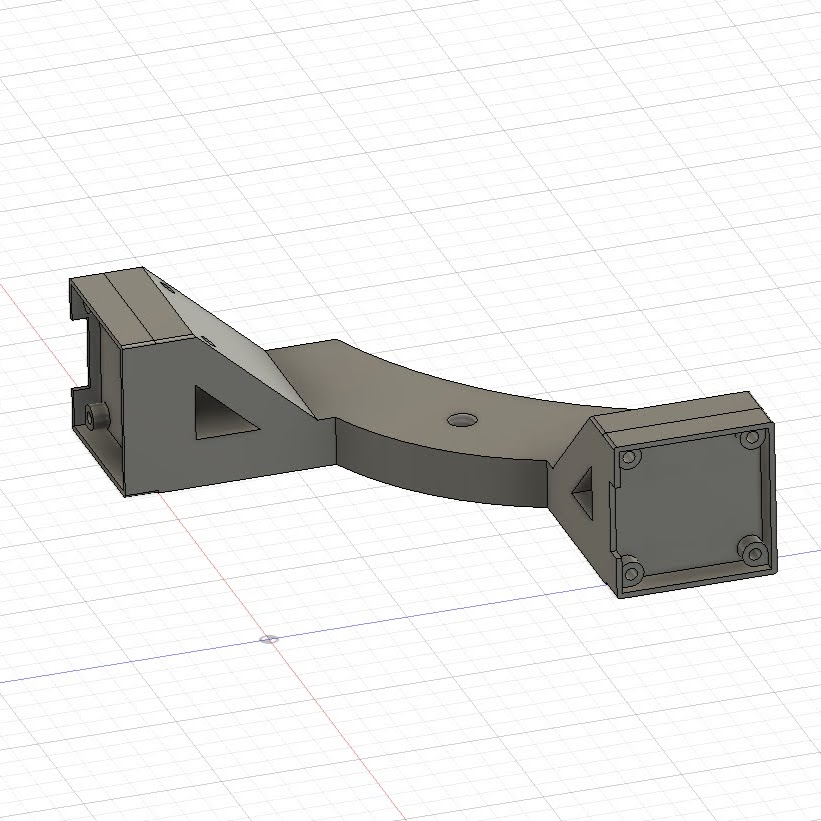
\includegraphics[width=\textwidth]{graphics/CAD.jpg}
    \caption{The CAD model of the prototype.}
    \label{fig:proto_scheme}
  \end{subfigure}
  \hfill
  \begin{subfigure}[b]{0.49\textwidth}
    \centering
    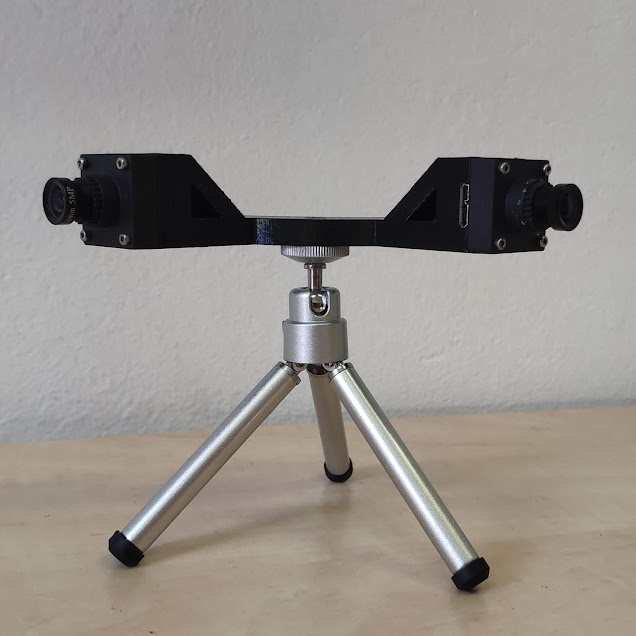
\includegraphics[width=\textwidth]{graphics/prototype.jpg}
    \caption{The printed prototype}
    \label{fig:proto_printed}
  \end{subfigure}
  \caption{The proposed sollution prototype.}
  \label{fig:prototype}
\end{figure}

CAD model of a camera mount was created in the Fusion360 software considering the requirements of a $90^\circ$ rotation between cameras and distance of the cameras close to the average MAV size.
A picture of the design from the CAD software is in \autoref{fig:proto_scheme}.
The 3D-printed prototype with the cameras mounted is in the \autoref{fig:proto_printed}

Basler daA1600-60um cameras were chosen for this project because they have a global shutter which is important when deployed onboard a fast-moving platform, good image quality and high framerate, making them suitable for the proposed method based on the assumptions defined in \autoref{sec:problem_definition}. 
More details regurding camera parameters are in \autoref{tab:daA1600}.

\begin{table}
    \begin{center}
      \begin{tabular}{ l l }
      \hline
      Parameter              & Value             \\ \hline
      Lens mount type        & S-mount           \\
      Data transfer protocol & USB 3.0           \\
      Max. frame rate        & 60 fps            \\
      Resolution (HxV)       & 1600 px x 1200 px \\
      Resolution             & 2 MP              \\
      Price                  & 289.00 EUR        \\ \hline
      \end{tabular}
    \end{center}
    \caption{daA1600-60um specifications.}
    \label{tab:daA1600}
\end{table}

Lenses of the cameras were chosen so that the resulting horizontal FOV is approximately $120^\circ$, which provides a sufficient overlapping zone to detect features in $\Psi$ (see \autoref{fig:sch_stereo}).

The solution was developed and tested on the Lenovo ThinkPad X280 with Intel(R) Core i7-8550U CPU and 16Gb RAM.
Intel NUC with Intel(R) Core i7-10710U CPU and 16Gb RAM is used as the onboard computer for the MAV.
No dedicated GPU is needed.

\section{Software tools}
\label{sec:impl_software}

The proposed solution uses the Robot operating system (ROS) \cite{Rospaper} as a middleware.
ROS is an open-source ecosystem with hundreds of already implemented algorithms and libraries to interact between different parts of a robot's system, such as sensor drivers, image processing algorithms, planners, controllers etc.
The AprilTag detector and a driver for Basler cameras used in this thesis are based on publicly available modules from the ROS community.

The MRS UAV system \cite{Baca2021} is used as a drone control environment. It is based on ROS, but it is a unique framework for MAVs to implement and test path planning, control, computer vision, object tracking, and many more MAV-related problems.

The OpenCV\footnote{\url{https://opencv.org/}} open-source computer vision library and the Eigen\footnote{\url{http://eigen.tuxfamily.org}} open-source library for efficient linear algebra were used for the implementation.
All of the software presented in this thesis was implemented in C++.

\begin{figure}[h]
    \centering
    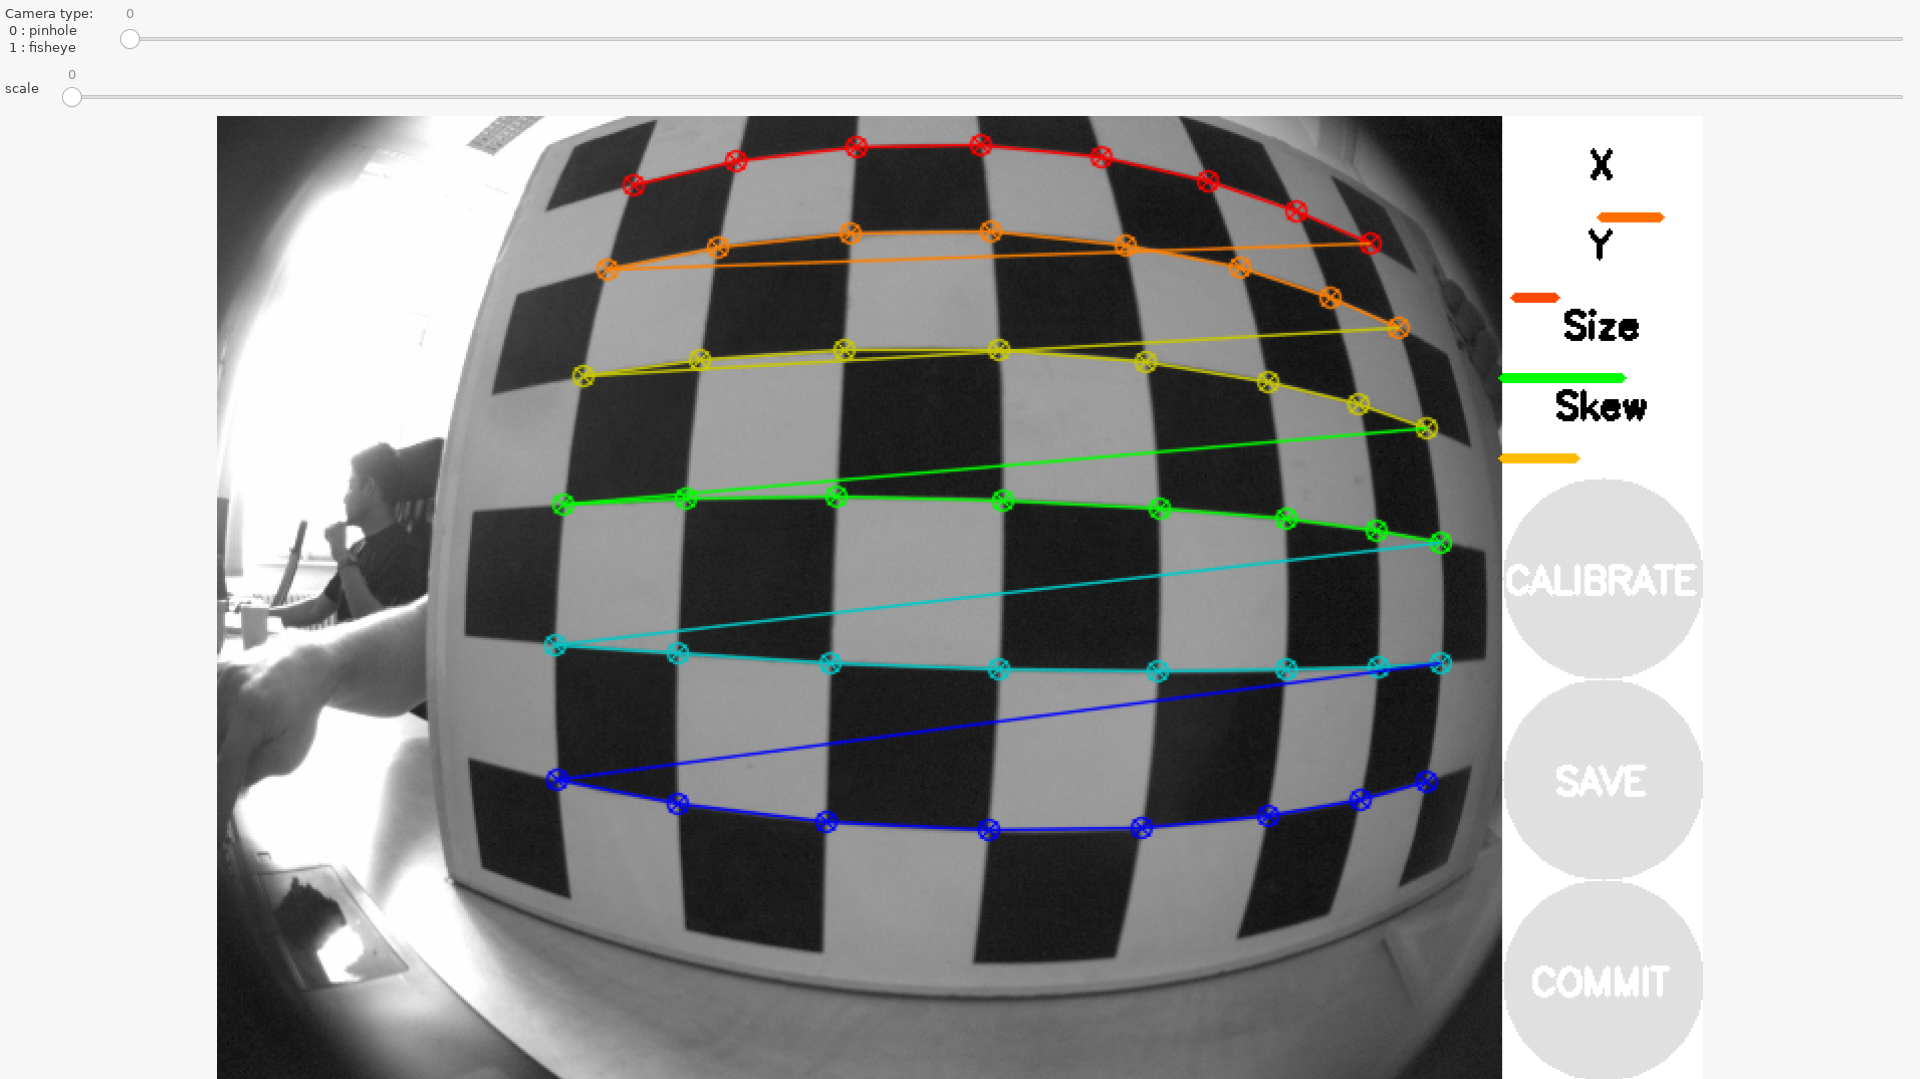
\includegraphics[width=.6\textwidth]{graphics/calibration.png}
    \caption{The single camera calibration process.}
    \label{fig:calib}
\end{figure}

Calibration of parameters od the camera projection and distortion models (described in \autoref{sec:meth_calib}) was performed using ROS camera calibration package\footnote{\url{http://wiki.ros.org/camera_calibration}}.
A chessboard pattern is used for the calibration, and its physical parameters must be specified to the calibration program.
The calibration process itself is done interactively using a graphical user interface (shown in \autoref{fig:calib}).
The interface displays the progress of the process to the user, and when a sufficient dataset is obtained, the user can trigger the parameter optimization. 
Results of the optimization are then saved to a file for later use.

\begin{figure}[h]
    \centering
    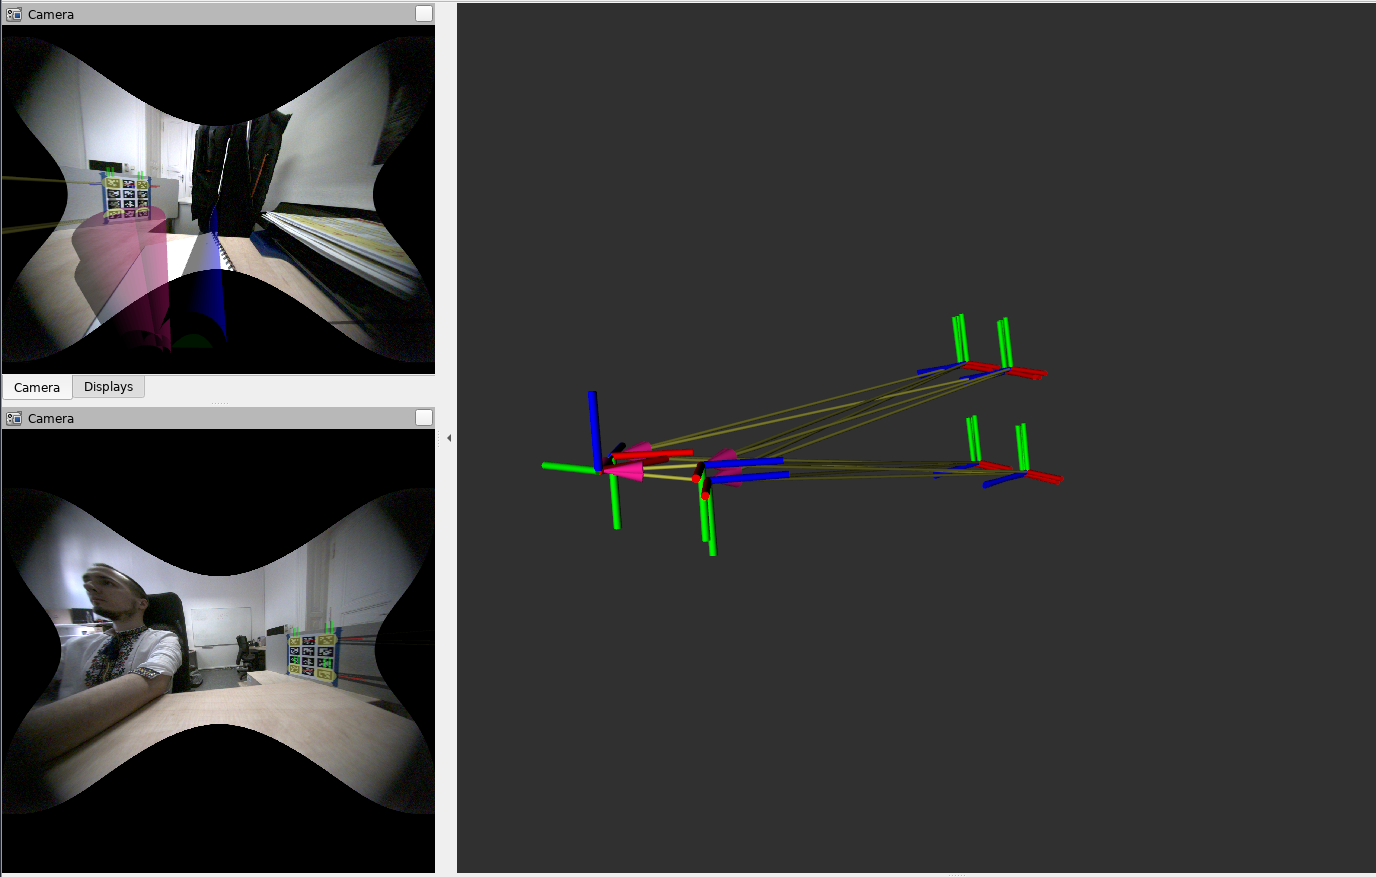
\includegraphics[width=.8\textwidth]{graphics/calib_process.png}
    \caption[The stereocamera calibration process]{The stereo pair calibration. In the left side there are views from the right camera (top) and left camera (bottom). Both cameras observing the AprilTag's pattern. On the right side there is a visualization from the ROS Vizualisation tool (rviz) of initial pozes of both cameras, AprilTags and the corrected right camera pose.}
    \label{fig:calib_stereo}
\end{figure}

The two calibration methods described in \autoref{sec:stereocalib} were both implemented to use an AprilTag calibration pattern, shown in \autoref{fig:aptags}.
The main reason why this pattern was chosen is that each tag can be detected individually, so there is no need to have all of them simultaneously in the overlapping zone.
The first method, described in \autoref{sec:lsq_umeyama}, is implemented using the "Least-square estimation of transformation between two point sets" \cite{Umeyama1991} implementation from Eigen.
Measurements from the CAD model of the camera mount were used as the initial estimate of the cameras' relative pose.
The second method, described in \autoref{sec:pnp}, is implemented using the OpenCV PnP solver.
Because the publicly available implementation of the AprilTag detector outputs only 3D poses of detected tags, the detector was modified to output also 2D coordinates of corners of the detected markers, which is needed for the PnP algorithm and during the debug session for computing the reprojection error.
The calibration process is in the \autoref{fig:calib_stereo}.

\begin{figure}[h]
  \begin{subfigure}[h]{0.49\textwidth}
    \centering
    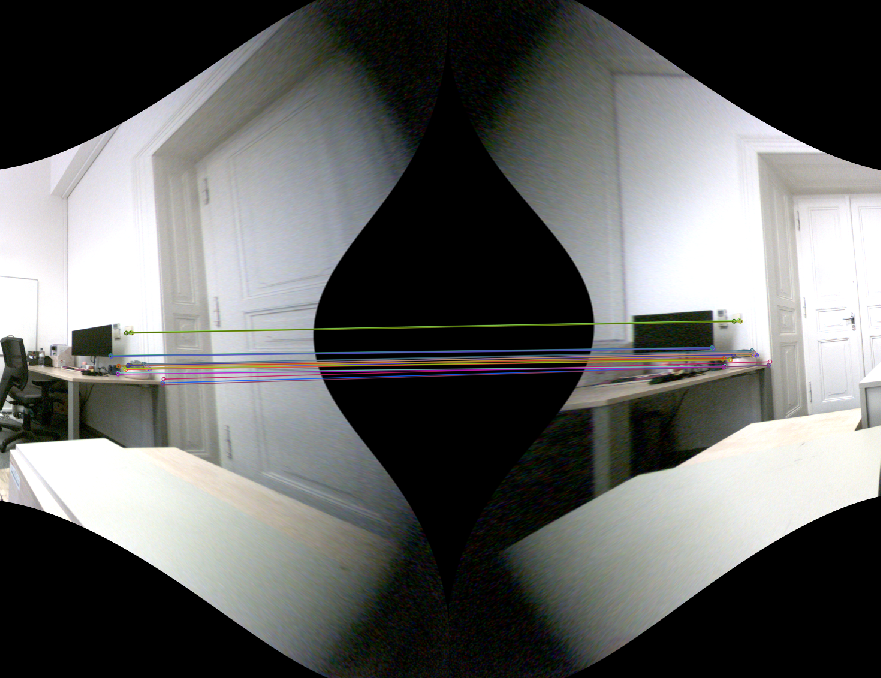
\includegraphics[width=0.92\textwidth]{graphics/corresp.png}
    \caption{The result of features detection, matching and outliers filtering.}
    \label{fig:corresp_life}
  \end{subfigure}
  \hfill
  \begin{subfigure}[h]{0.49\textwidth}
    \centering
    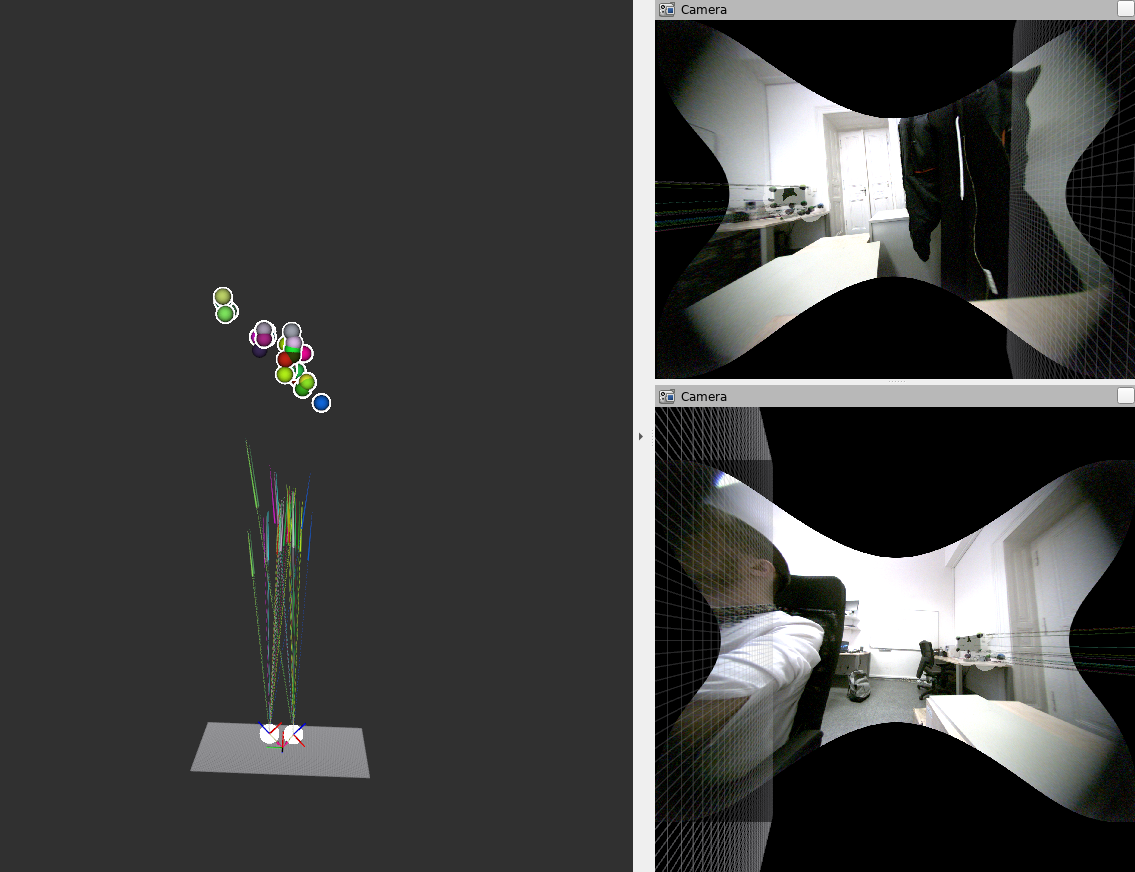
\includegraphics[width=\textwidth]{graphics/res_trangulation.png}
    \caption{Triangulated points}
    \label{fig:triang_life}
  \end{subfigure}
  \caption{}
  \label{fig:res}
\end{figure}

After both cameras and the stereo pair are calibrated, the following steps are feature detection, matching and filtering, described in \autoref{sec:features}, for a synchronized pair of images. 
The example from a real experiment is in \autoref{fig:corresp_life}.

The synchronization is done on the stereo pair driver level.
As described in \autoref{sec:features}, the ORB detector and a brute-force matcher implementation from the OpenCV were used for feature detection and matching.
The next step is reconstructing the 3D scene from the obtained feature pairs.
The method described in \autoref{sec:shortest_distance} is implemented from scretch, and the implementation of triangulation described in \autoref{sec:svdtriang} is taken from the OpenCV.
In the \autoref{fig:triang_life} in the left part there are triangulated points shown as colored spheres, and rays pointing from camera centers to feature points colored with the same color as corresponding feature.
In the right side there are cameras' views.


% As a result, obstacles in the cameras' overlapping zone are detected in a format of the point cloud and correspondent feature points on both images.
% Recalling the \autoref{fig:intro_general}, the proposed solution providing a pointcloud with obstacles in a red zone at each timestamp $t_i$. 
